\documentclass[11pt,a4paper]{ivoa}
\input tthdefs

\usepackage{array}
\usepackage{tabulary}  % for nicer tables
\usepackage{calc}
\usepackage{placeins}
\setlength\extrarowheight{2pt}

\newcolumntype{L}{>{\centering\arraybackslash}m{3cm}}

\title{Model Instances in Votables}

% see ivoatexDoc for what group names to use here
\ivoagroup{DM}

\newcommand{\TODO}[1]{%
    \noindent%
    \colorbox{todocolor}{%
            \parbox{0.85\linewidth}{\sffamily \textbf{TODO:}\\
            #1}
    }%
    \vspace{2pt}

}

\newcommand{\note}[1]{%
    \noindent%
    \textcolor{darkgrey}{{\sffamily Note:} \emph{#1}}%
}

\newcommand{\comment}[1]{%
    \noindent%
    \textcolor{red}{{\sffamily Comment:} \emph{#1}}%
}

\definecolor{todocolor}{rgb}{1,1,0.8}
\definecolor{darkred}{rgb}{0.6,0,0}
\definecolor{rose}{rgb}{1.0,0.88,0.88}
\definecolor{darkgrey}{rgb}{0.35,0.35,0.35}
\definecolor{gray}{rgb}{0.4,0.4,0.4}
\definecolor{darkblue}{rgb}{0.0,0.0,0.6}
\definecolor{maroon}{rgb}{0.5,0,0}
\definecolor{cyan}{rgb}{0.0,0.6,0.6}

\lstset{
  basicstyle=\ttfamily,
  columns=fullflexible,
  showstringspaces=false,
  commentstyle=\color{gray}\upshape
}

\lstdefinelanguage{XML}
{
  morestring=[b]",
  morestring=[s]{>}{<},
  morecomment=[s]{<?}{?>}, 
  morecomment=[s]{<!--}{-->},
  stringstyle=\color{black},
  identifierstyle=\color{darkblue},
  keywordstyle=\color{maroon},
  morekeywords={ref,utype,dmrole, dmtype, value}% list your attributes here
}

\lstdefinestyle{XML}{
    captionpos=b,
    basicstyle=\small\ttfamily
}
\author{François Bonnarel}
\author{Gilles Landais}
\author{Laurent Michel}
\author{Jesus Salgado}

\editor{Laurent Michel}

% \previousversion[????URL????]{????Concise Document Label????}
\previousversion{This is the first public release}
       

\begin{document}

\begin{abstract}
Vodml-instance-vot proposes a syntax to map VOTable data on any model serialized in VO-DML.
Vodml-instance-vot annotations are grouped in a single XML block located in the VOTable head. The annotation block allows to easily reconstruct the model structure. It designed in a way that the block can be reused on different data sets in order to facilitate the annotation process.
Vodml-instance-vot is enable to join data from different tables
\end{abstract}


\section*{Acknowledgments}
CDS/TDIG/SourceDM contributors

\section*{Conformance-related definitions}

The words ``MUST'', ``SHALL'', ``SHOULD'', ``MAY'', ``RECOMMENDED'', and
``OPTIONAL'' (in upper or lower case) used in this document are to be
interpreted as described in IETF standard RFC2119 \citep{std:RFC2119}.

The \emph{Virtual Observatory (VO)} is a
general term for a collection of federated resources that can be used
to conduct astronomical research, education, and outreach.
The \href{http://www.ivoa.net}{International
Virtual Observatory Alliance (IVOA)} is a global
collaboration of separately funded projects to develop standards and
infrastructure that enable VO applications.


\section{Introduction}
The first purpose of a model is to provide,  for a particular domain, a formal description of the relevant quantities and of the way they are connected together .
This documentary role facilitates the communication between the stack-holders and thus the design of interoperability protocols. 

At data level, interoperability consists in arranging searched data in a way that a client can understand them without taking care of their origin. So that, the same code can process and compare data coming from different sources.  That way to arrange data is given by the model.

This is not done by default with VOtables because VOTables are containers. The VOTable schema cannot say how data are mapped on a given model or whether they match any model at all. This is not an issue for simple protocol responses (ref) because the VOTable structure is defined by the protocol itself. This is however a big issue for VOTables containing native data such as Vizier  or TAP query responses.

The challenge here is to bind native data with a given model in a way that a model aware software can see them as model instances while maintaining the possibility to access them in their original forms.

This is partially done with UTypes which may connect FIELDs or PARAMs with model leaves in the case of simple tree-views of the model. Unfortunately, there is nos unique  way to build and parse UTypes in the context of complex models. This occurs when e.g the same class is used in different location of the model or when the model contains loops. It is also not possible to refer data from different tables with  UTypes.

%Fb : "This is just because UTypes have been invented at a period when there was no standard way to formally describe  models." Actually it's more complex than that. As long as the model instances are flat or simple trees (charcaterisation) utypes may work. When you have some loops (like in complex Provenace queries) utypes are not enough to map the structure of instances (corrected LM)

The landscape has dramatically changed in 2016 when VODML (ref) became a recommendation. VODML is a meta-model that gives a standard way to express VO models and to make them machine-readable.
%FB: if we have the reference we don't need "which is a rec since é016" (fixed LM)
In VODML, model leaves are no longer identified by a simple string like UTypes do but by a certain role played in a given location in the model hierarchy.
The consequence is that any annotation mechanism based on VODML will preserve the model hierarchy to save the role played by any components. In this context, it might be easy to re-construct model instances from the annotations. 
%FB: see above the actual difference between utype strategy and vodml lite mapping (fixed LM)
%FB : I don't understand at all following sentence "This is very interesting because a copy that model hierarchy with leaves set with real data is nothing else that a model instance which is exactly what we need to be interoperable." (fixed LM)

The main concept of this standard is to insert on the  top of the VOTable an XML block compliying with the model structures and containing references to the actual data.
In such a way that a model-aware client only has to make a copy of that structure and to resolve the references  to build an instance. More generic model-unaware clients can just ignore the mapping block. 
This approach, proposed by (GL and OL), allows a perfect restitution of the model from the annotation, a round-trip validation. It follows a real ORM schema actually.
Our approach is a bit different. From our use case perspective (see below), clients do not need  to care about the difference between data types and object types or between relations and compositions or some other finesses. They need to be able to reconstruct a browable data hierarchy. The can be done by assembling key/vakues pairs, tuples and arrays. This way to serialize complex data is used with a great success by most of the Web applications working with JSON/YAML messages. 
Our bet is that the loss of certain features of the model will allow significant gain in readability, and thus in reliability, while facilitating the work of annotation. 
The proposed syntax renders the data hierarchy with three elements sibling to the JSON concepts (ATTRIBUTE as key/vakue pair, INSANCE as tuple and COLLECTIONS as arrays). In addition to this, some other elements have been added to guide the parse. 
The connection with the data is made with element attributes in order to keep the structure of the XML elements independant from the data layout.

These ideas were first tested first in the framework of the TDIG on VOTABLEs containing time series provided by different missions such as Gaia or ZWICKI. 
Then, the syntax has been refined to be used to validate the Mango model on real data.


\lstset{language=XML}

\subsection{Role within the VO Architecture}

\begin{figure}
\centering

% As of ivoatex 1.2, the architecture diagram is generated by ivoatex in
% SVG; copy ivoatex/archdiag-full.xml to archdiag.xml and throw out
% all lines not relevant to your standard.
% Notes don't generally need this.  If you don't copy archdiag.xml,
% you must remove archdiag.svg from FIGURES in the Makefile.

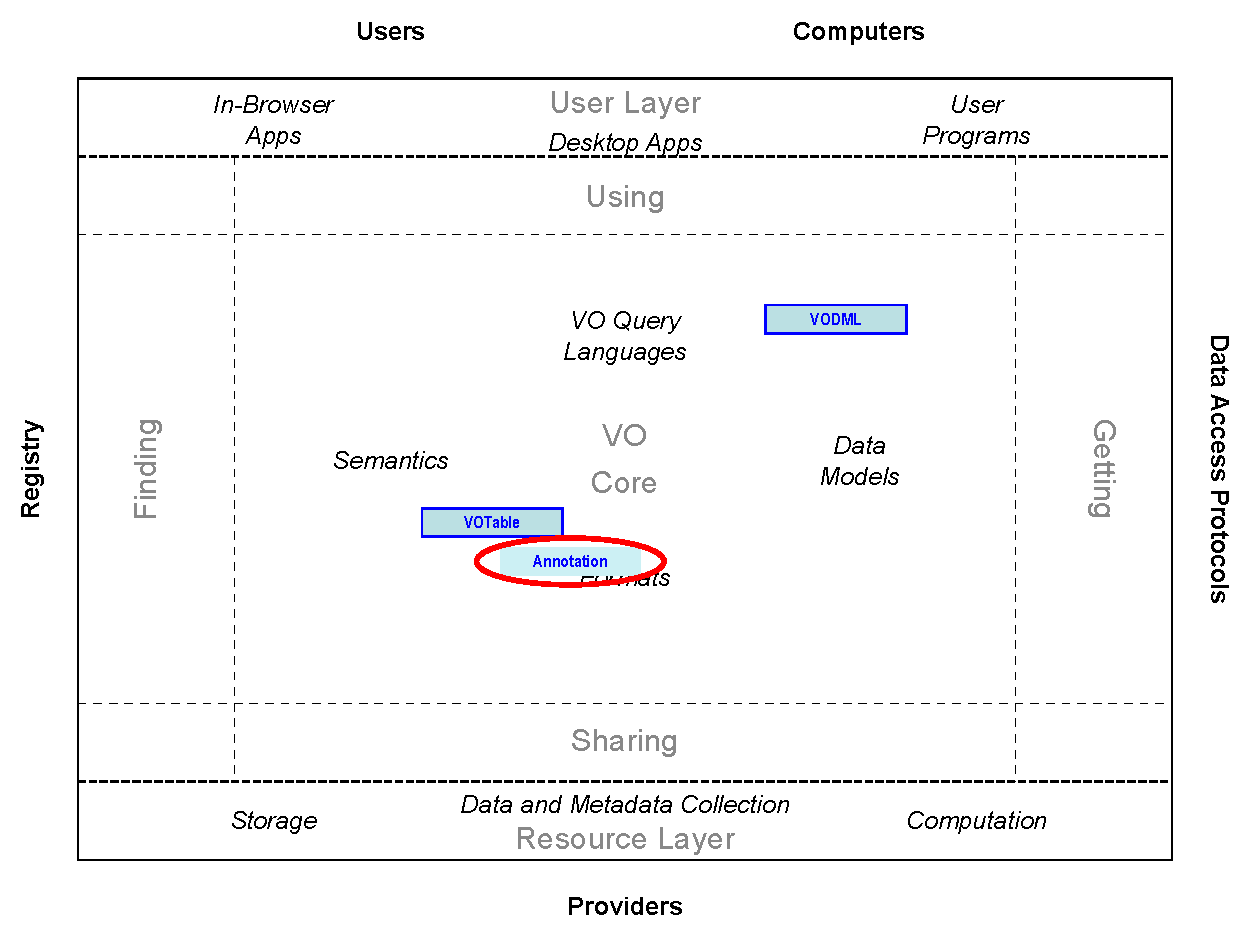
\includegraphics[width=0.9\textwidth]{role_diagram.pdf}
\caption{Architecture diagram for this document}
\label{fig:archdiag}
\end{figure}

Fig.~\ref{fig:archdiag} shows the role this document plays within the
IVOA architecture \citep{note:VOARCH}.

???? and so on, LaTeX as you know and love it. ????

\section{Use Cases and Requirement}

\subsection{Use Cases}

\subsubsection{Client Side}

The mapping is self consistent. Its role is to give the client all information it needs to reconstruct a datastructure compliant with the model. 
A model-aware client must be able to do this without implementing model-specific  code.  
%The mapping syntax is independant of the model. The structure of the mapped model is given by the arrangement of the mapping elements, not by the elements themselves

\textbf{Identifying the nature of the content of a VOTable}:  A client can check the annotation block of a VOTable to decide how to process it. For instance, it can detect that the VOTable contains a Provenance instance  and then invoke a specific viewer. 

\textbf{Measurement discovery}: A client wants to discover whether a VOTable contains some peculiar measurements (position, velocity...). This can be done with a quick parsing of the annotation block.

\textbf{Data set comparison}: A client wants to compare different data set s (e.g. Xmatch, plot). The annotation provides a homogeneous data representation that allows to put them together in a consistent way. 

\textbf{Data set export}: A client wants to export (e.g. with SAMP) a model instance in a convenient format (e.g. json). The JSON model instance can be buit from the annotation block and exported to a another party.

\subsubsection{Server Side}
The server use cases are to make possible the realization of those of the clients  for a reasonable cost. The annotation process can represent a significant extra work for the curator team that must be limited as much as possible. To do so the mapping syntax is designed to facilitate the use of templates and components.

3 server types that could annotate data have been identified:
\begin{enumerate}
   \item \textbf{Mission data provider}: the data annotation can be set once forever for each data product at the design phase.
   \item \textbf{Archival data provider}: The data annotation must be done for each archived datat set. 
           The curator has a little control, on the data format and he/she has to do his best to match data with the model(s).
           In this case, it must be possible limit the annotation on a subset of data.
   \item \textbf{TAP data provider}: In case of TAP services, the annotation process is in charge of the TAP server that must dynamically match queried data with model quantities, and this for each specific query.
\end{enumerate}

The goal of this version of the specification is to support requirements 1) and 2) with a special attention to make 2) easier. 
Support of requirement 3) is still an experimental feature at the time this specification is written.


\subsection{Requirements}

\begin{itemize}
\item Shy Annotations: The data mapping must not affect the operation of existing clients.

\item Faithful Annotations: The structure of the annotation must be faithful to any VODML compliant model. 


\item Different Usage Levels 
\begin{itemize}
   \item The data mapping must be easily ignored by the client.
   \item The data mapping must allow clients to easily detect the model on which data are mapped.
   \item The data mapping must allow clients to easily get the general metadata (e.g. coordinate systems).
   \item The data mapping must allow clients to get full model instances for each table row.
\end{itemize}

\item Easy to Build 
\begin{itemize}
   \item The mapping structure must be independent of the data structure.
   \item The mapping syntax should make easy the building of both mapping components and templates.
\end{itemize}

\item Complex Data Mapping 
\begin{itemize}
   \item The mapping syntax must able to annotate data spread over several tables.
   \item The mapping syntax must be able to filter data rows that have to be instanciated.
   \item The mapping syntax must be able to group data rows in an set of instances.
\end{itemize}
\end{itemize}


\section{Syntax}


The syntax rules specified in this standard allow to build consistent annotations for any model. However, they do not prevent to do foolish things in the same way that a programming language grammar does not protect people against writing irrelevant software.
In the following annotation snippets, the values of the XML elements attribute do not refer toi any particular model or VOTable. They have been choosen to help readers to figure out their meanings.

\subsection{Mapping Block Structure}

The mapping block muts be the direct child of \texttt{VOTABLE}. Its scope is the whole VOTable. Its stucture is given below.

\begin{lstlisting}[caption={INSTANCE bloc example},style=XML]
<VOTABLE xmlns="http://www.ivoa.net/xml/VOTable/v1.3" 
            xmlns:xsi="http://www.w3.org/2001/XMLSchema-instance" 
            version="1.4">
   <MODEL_INSTANCE>
     <MODELS>   ...  </MODELS>
     <GLOBALS>   ...  </GLOBALS>

      <TABLE\_MAPPING tableref=...>  ... </TABLE\_MAPPING tableref=...>
      <TABLE\_MAPPING tableref=...> ...  </TABLE\_MAPPING tableref=...>
    ...
   </MODEL_INSTANCE>
   ..
</VOTABLE>
\end{lstlisting}

The mapping construction rules are the same whatever either model or data layout are.

\begin{itemize}
    \item The mapping is located in a \texttt{<MODEL\_INSTANCE>} block, child of \texttt{<VOTABLE>}.
    \item The mapping elements denote the model structure.
    \item The \texttt{<MODEL\_INSTANCE>} block starts with the list of implemented models.
    \item The model list is followed the \texttt{<GLOBALS>} block containing data shared by the whole mapping.    
    \item The \texttt{<GLOBALS>} block is followed a sequence of \texttt{<TABLE\_MAPPING>}.
    \item There is one \texttt{<TABLE\_MAPPING>} per mapped \texttt{<TABLE>}.
\end{itemize}
\FloatBarrier

%%%%%%%%%%%%%%%%%%%%%%%%%%%%%%%%%%%%%
%
% TOP LEVEL STRUCTURE
%
%%%%%%%%%%%%%%%%%%%%%%%%%%%%%%%%%%%%%

\subsection{Mapping Top Level Structure}
%%%%%%%%%%%%%%%%%%%%%%%%%%%%%%%%%%%%%
%
% MODELS
%

\subsubsection{MODELS}

The  \texttt{MODELS}  blocks contains the list of the models mapped in the block. 


\begin{itemize}
    \item The model list is informative, it is not requested to achieve the parsing.
    \item The model list can be left empty.
    \item Models referenced in \texttt{MODELS} are not necessary VO standards, but they must be accessible by a VODML URI
\end{itemize}

\begin{lstlisting}[caption={GLOBALS block example},style=XML]
<MODELS>
    <MODEL>
        <NAME>ivoa</NAME>
        <URL>http://www.ivoa.net/xml/VODML/IVOA-v1.vo-dml.xml
        </URL>
    </MODEL>
    <MODEL>
        <NAME>coords</NAME>
        <URL>http://www.ivoa.net/xml/STC_coords-v1.0.vo-dml.xml
    </URL>
    </MODEL>
    <MODEL>
        <NAME>meas</NAME>
        <URL>http://www.ivoa.net/xml/STC_meas-v1.0.vo-dml.xml
        </URL>
    </MODEL>
</MODELS>
\end{lstlisting}

 \texttt{MODELS},  {MODEL},  {NAME} and {URL}  have no attributes. 
 \FloatBarrier

%%%%%%%%%%%%%%%%%%%%%%%%%%%%%%%%%%%%%
%
% GLOBALS
%

\subsubsection{GLOBALS}
 Contains  \texttt{INSTANCE}s  that can be used everywhere in the \texttt{MODEL\_INSTANCE}.

\begin{itemize}
    \item \texttt{INSTANCE}s children of \texttt{GLOBALS} should have an  \texttt{@ID} attribute so that they can be referenced from other instances.
    \item The role of the \texttt{GLOBALS}s children, (\texttt{INSTANCE}s by construction), must be ignored although being mandatory.
    \item References within \texttt{GLOBALS}s  sub-elements to VOTable data (\texttt{FIELD} ot \texttt{PARAM}) must be searched in all tables. 
            They must be resolved by the first occurence matching the reference found.
    \item \texttt{GLOBALS} has no attributes. 
\end{itemize}

\begin{lstlisting}[caption={GLOBALS block example},style=XML]
  <GLOBALS>
    <INSTANCE ID="SpaceCoordFrame" >
      <INSTANCE dmrole="coords:SpaceFrame.refPosition" 
                 dmtype="coords:StdRefLocation">
          <ATTRIBUTE dmrole="coords:StdRefLocation.position" 
                      dmtype="ivoa:string" value="NoSet"/>
      </INSTANCE>
      <ATTRIBUTE dmrole="coords:SpaceFrame.spaceRefFrame" 
                  dmtype="ivoa:string" value="ICRS"/>
      <ATTRIBUTE dmrole="coords:SpaceFrame.equinox" 
                  dmtype="coords:Epoch"   value="NoSet"/>
    </INSTANCE>
 </GLOBALS>
\end{lstlisting}




\begin{table}[!htbp]
\small
\centering
\begin{tabulary}{\linewidth}{|c|J|}       
       \hline 
           \textbf{Child} &  
           \textbf{Role}\\
       \hline         \hline  
            \texttt{INSTANCE}    &  
            Model instances with a scope covering the whole VOTable . \\       
       \hline 
     \end{tabulary}
     \caption{Allowed  \texttt{GLOBALS} children} 
     \label{tbl:globals-children}
 \end{table}

\FloatBarrier
%%%%%%%%%%%%%%%%%%%%%%%%%%%%%%%%%%%%%
%
% TABLE\MAPPING
%

\subsubsection{TABLE\_MAPPING}

\texttt{TABLE\_MAPPING} blocks contain the mapping statements of the data contained in one \texttt{TABLE} .

\begin{itemize}
    \item There is one \texttt{TABLE\_MAPPING} block for each mapped \texttt{TABLE}  in the VOTAble.    
    \item A \texttt{TABLE} cannot be referenced by more than one \texttt{TABLE\_MAPPING} element.
    \item The table related to a \texttt{TABLE\_MAPPING} is identified by the @\texttt{tableref} attribute. 
            It must be first resolved against the \texttt{TABLE} identifier ( @\texttt{ID} ) and then against the table name.
\end{itemize}

\begin{lstlisting}[caption={TABLE\_MAPPING block example},style=XML]
<TABLE_MAPPING tableref="OtherResults">
    <COLLECTION dmrole="test:detections">
        <TABLE_ROW_TEMPLATE>
            <INSTANCE dmrole="" dmtype="test:Detection">
               <ATTRIBUTE dmrole="test:detection.num" dmtype="ivoa:real"
                           ref="_num_148" />
               <ATTRIBUTE dmrole="test:detection.id" dmtype="ivoa:real"
                           ref="_foreign" />
           </INSTANCE>
        </TABLE_ROW_TEMPLATE>
    </COLLECTION>
</TABLE_MAPPING>
\end{lstlisting}


\begin{table}[!htbp]
\small
\centering
\begin{tabulary}{\linewidth}{|c|J|}       
       \hline 
           \textbf{Child} &  
           \textbf{Role}\\
       \hline         \hline  
           \texttt{INSTANCE}    & 
           Mapping of an object or a data type.  \\              
       \hline  
            \texttt{TABLE\_ROW\_TEMPLATE}    &  
            One instance must be built for each table row. 
             \newline The structure of those instances is given by the TABLE\_ROW\_TEMPLATE children \\              
       \hline  
             \texttt{COLLECTION}    &  
             Mapping of an object collection \\       
       \hline 
     \end{tabulary}
     \caption{Valid \texttt{TABLE\_MAPPING} children} 
     \label{tbl:templ-children}
 \end{table}


\begin{table}[!htbp]
\small
\centering
\begin{tabulary}{\linewidth}{|c|J|}       
       \hline 
            \textbf{Attribute} & 
            \textbf {Role}\\
       \hline         \hline  
            @tableref  & 
            The @ID or the @name of the mapped table  \\
       \hline 
     \end{tabulary}
     \caption{\texttt{TABLE\_MAPPING} attributes} 
     \label{tbl:templ-att}
 \end{table}

\begin{table}[!htbp]
\small
\centering
\begin{tabulary}{\linewidth}{|c|c|c|c|J|}
    \hline 
        \textbf{@tableref} &
        \textbf{Pattern}\\
    \hline      \hline  
        MAND &   
        Always mandatory\\
   \hline 
\end{tabulary}
     \caption{Valid attribute patterns for  \texttt{TABLE\_MAPPING}} 
     \label{tbl:templ-pattern}
 \end{table}
\FloatBarrier

%%%%%%%%%%%%%%%%%%%%%%%%%%%%%%%%%%%%%
%
% DATA HIERARCHY
%
\subsection{Data Hierarchy}

%%%%%%%%%%%%%%%%%%%%%%%%%%%%%%%%%%%%%
%
% INSTANCE
%

\subsubsection{INSTANCE}

Mapping for either object types or a datatype instances.

\TODO{ put a better rexample}

\begin{lstlisting}[caption={INSTANCE block example},style=XML]
<INSTANCE dmrole="ds:Dataset.dataID" dmtype="ds:DataID">
    <ATTRIBUTE dmrole="ds:DataID.title" value="Gaia TS Mapping Test" />
    <ATTRIBUTE dmrole="ds:DataID.datasetID" value="ivoa://gaia/ts/12345" />
    <ATTRIBUTE dmrole="ds:DataID.creatorDID" value="ivoa://esa/gaia/" />
    <ATTRIBUTE dmrole="ds:DataID.version" value="0.0" />
    <ATTRIBUTE dmrole="ds:DataID.date" value="2018:11:11" />
    <ATTRIBUTE dmrole="ds:DataID.creationType" value="LiteMappingTest" />
    <INSTANCE dmrole="ds:DataID.creator" dmtype="ds:Creator">
        <INSTANCE dmrole="ds:Role.party" dmtype="ds:party.Individual">
            <ATTRIBUTE dmrole="ds:Party.name" value="MODEL_INSTANCE-Team" />
       </INSTANCE>
    </INSTANCE>
</INSTANCE>
\end{lstlisting}


\begin{table}[!htbp]
\small
\centering
\begin{tabulary}{\linewidth}{|c|J|}       
       \hline 
           \textbf{Child} &  
           \textbf{Role} \\
       \hline         \hline  
           \texttt{INSTANCE}    & 
           Another embedded instance . \\       
       \hline  
           \texttt{ATTRIBUTE}    & 
           Primitive attribute . \\       
       \hline  
            \texttt{COLLECTION}    & 
           Set of items\\      
       \hline 
     \end{tabulary}
     \caption{Valid  \texttt{INSTANCE} children} 
     \label{tbl:inst-chilrdren}
\end{table}

\begin{table}[!htbp]
\small
\centering
\begin{tabulary}{\linewidth}{|c|J|}       
       \hline 
            \textbf{Attribute} &  
            \textbf{Role}\\
       \hline  
            @dmrole    & 
            VODML role.  \newline Can be empty if located in GLOBALS or in TABLE\_ROW\_INSTANCE \\
       \hline  
            @dmtype & 
            VODML type of the instance.  \newline Must never be empty \\
       \hline  
            @dmref  & 
            Reference to another instance in the mapping block. 
            \newline  Must never be empty\\          
       \hline  
            @ID  & 
            Unique identifier of the instance. 
            \newline  Must never be empty\\
       \hline 
     \end{tabulary}
     \caption{\texttt{INSTANCE} attributes} 
     \label{tbl:inst-att}
 \end{table}

\begin{table}[!htbp]
\small
\centering
\begin{tabulary}{\linewidth}{|c|c|c|c|J|}
    \hline 
        \textbf{@dmrole} & 
        \textbf{@dmref} &  
        \textbf{@dmtype} &  
        \textbf{@ID} &  
        \textbf{Pattern}\\
    \hline      \hline  
        MAND &   
       & 
       MAND & 
       OPT & 
       Instance of a certain type playing a certain role. \\
    \hline  
       MAND  & 
       MAND  &  
       &  
       & 
       Reference to another instance. 
        \newline  No allowed children in this case.  \\
      \hline 
\end{tabulary}
     \caption{Valid attribute patterns for  \texttt{INSTANCE}} 
     \label{tbl:inst-pattern}
 \end{table}
\FloatBarrier
%%%%%%%%%%%%%%%%%%%%%%%%%%%%%%%%%%%%%
%
% ATTRIBUTE
%

\subsubsection{ATTRIBUTE}

Mapping statement for primitive attributes.

\begin{itemize}
    \item \texttt{ATTRIBUTE}s  are the model leaves.     
    \item \texttt{ATTRIBUTE}  values can either be set by reference on tabke data or by literal values. 
    \item \texttt{ATTRIBUTE}s have no children.
\end{itemize}

\begin{lstlisting}[caption={ATTRIBUTE examples},style=XML]
<INSTANCE dmrole="model:value.example" dmtype="model:value.Example">
    <ATTRIBUTE dmrole="model:preset.value" value="Preset Value" />    
    <ATTRIBUTE dmrole="model:ref.value" ref="fieldID" />    
    <ATTRIBUTE dmrole="model:reforpreset.value" 
                value="Preset Value" ref="fieldID" />
</INSTANCE>
\end{lstlisting}


\begin{table}[!htbp]
\small
\centering
\begin{tabulary}{\linewidth}{|c|J|}
       \hline 
          \textbf{Attribute} & 
          \textbf{Role}\\
       \hline         \hline  
          @dmrole    & 
           VODML role of the attribute. 
           \newline  Must never be empty\\       
       \hline 
          @dmtype    & 
          VODML type of the instance attribute.
           \newline  Must never be empty\\
       \hline  
          @value   &
          Literal value of the instance attribute. 
                     \newline If  \texttt{ATTRIBUTE} has also a \texttt{@ref}, \texttt{@ref} MUST be resolved first.
                     \texttt{ATTRIBUTE}  \texttt{@val} must be taken when \texttt{@ref} cannot be resolved \\
        \hline
           @ref & 
            Reference of the data element (\texttt{FIELD} or \texttt{PARAM}).  
                    \newline Must refer to an element of the \texttt{TABLE}  referenced by the current     
                    \texttt{TABLE\_MAPPING}                    
                    \newline The client MUST first look for a \texttt{FIELD} matching \texttt{@ref}. 
                    \newline If no \texttt{FIELD}  is found, it must look for a \texttt{PARAM}
                    \\
       \hline 
     \end{tabulary}
     \caption{\texttt{ATTRIBUTE} attributes} 
     \label{tbl:att-att}
 \end{table}

\begin{table}[!t]
\small
\centering
\begin{tabulary}{1.0\linewidth}{|c|c|c|c|J|}

    \hline    
          \textbf{@dmrole}  &  
          \textbf{@dmtype} &  
          \textbf{@ref} &  
          \textbf{@value} &  
          \textbf{Pattern}\\
    \hline   \hline 
          MAND & 
          MAND &  
          MAND &  
          OPT & 
          The instance attribute must take the value pointed by \texttt{@ref}. 
           \newline If the reference cannot be resolved, the attribute takes the value of \texttt{@val} if present.\newline  It is considered as not set otherwise.   \\
     \hline  
          MAND & 
          MAND &   
          &  
          MAND & 
          The attribute takes the value of \texttt{@val}.   \\
     \hline 
  \end{tabulary}
  \caption{Valid attribute patterns for  \texttt{ATTRIBUTE}} 
  \label{tbl:att-pattern}
 \end{table}
\FloatBarrier


%%%%%%%%%%%%%%%%%%%%%%%%%%%%%%%%%%%%%
%
% COLLECTION
%

\subsubsection{COLLECTION}

Mapping statement fort sets of either instances or collections.

\begin{itemize}
    \item A \texttt{COLLECTION} can contain a fixed set of instances or collections. 
            In this case, each element must be mapped individually.  
            Elements can be either \texttt{INSTANCE}s or \texttt{COLLECTION}s.
    \item A \texttt{COLLECTION} can contain an unbounded set of instances, one per selected table row. 
            In this case, all items have the same type and thus the same mapping. 
           They can be set with local table  data or with data from a joint table.
 \end{itemize}

The example below show up a a fixed length \texttt{COLLECTION}.

\begin{lstlisting}[caption={\texttt{COLLECTION} example},style=XML]
<TABLE\_MAPPING tableref="Results">
    <COLLECTION dmrole="meas:Measure.errors" size="2">
         <INSTANCE dmref="globals_stat_error" />         
         <INSTANCE dmref="globals_sys_error" />
    </COLLECTION>
</TABLE\_MAPPING>
\end{lstlisting}

\begin{table}[!htbp]
\small
\centering
\begin{tabulary}{\linewidth}{|L|J|}
       \hline 
           \textbf{Child} &
           \textbf{Role}\\
       \hline  \hline
           \texttt{INSTANCE}    & 
           Mapping of one collection item. A collection can embed multiple \texttt{INSTANCE}s \\              
       \hline  
           \texttt{COLLECTION}    & 
           Mapping of one collection item. A collection can embed multiple \texttt{COLLECTION}s \\              
       \hline  
           \texttt{TABLE\_ROW\_TEMPLATE}    & 
          The collection is populated with with one instance per row of the current table. When present, this element must be the only child. \\       
       \hline  
          \texttt{JOIN}    & 
         The collection is populated with data read from another table. When present, this element must be the only child.\\      
       \hline 
\end{tabulary}
\caption{Valid  \texttt{COLLECTION} children} 
\label{tbl:coll-children}
\end{table}

\begin{table}[!htbp]
\small
\centering
\begin{tabulary}{\linewidth}{|L|J|}
       \hline 
           \textbf{Attribute} & 
           \textbf{Role}\\
       \hline  \hline
          @dmrole    & 
           Role played by the collection (VODML relation name usually). Cannot be empty.\\       
       \hline  
          @size    & 
          Collection size. This attribute is not necessary to parse the mapping block.\\       
       \hline 
 \end{tabulary}
 \caption{Valid attributes for  \texttt{COLLECTION}} 
 \label{tbl:att-att}
 \end{table}


\begin{table}[!t]
\small
\centering
\begin{tabulary}{\linewidth}{|L|L|J|}
    \hline 
        @dmrole   & 
        @size   &  
        Role\\
    \hline  \hline
       MAND & 
       OPT & 
       Role played by the collection (VODML relation name usually). Cannot be empty \\    
    \hline 
  \end{tabulary}
  \caption{Valid attribute patterns for  \texttt{COLLECTION}} 
  \label{tbl:coll-pattern}
 \end{table}`
\FloatBarrier

%%%%%%%%%%%%%%%%%%%%%%%%%%%%%%%%%%%%%
%
% PARSING STATEMENTS
%
%%%%%%%%%%%%%%%%%%%%%%%%%%%%%%%%%%%%%
\subsection{Parsing Statement}

%%%%%%%%%%%%%%%%%%%%%%%%%%%%%%%%%%%%%
%
% TABLE_ROW_TEMPLATE
%

\subsubsection{TABLE\_ROW\_TEMPLATE}
This element indicates that one element must be added to the host \texttt{COLLECTION} for each table row.

\begin{itemize}
    \item The row mapping is given by the \texttt{INSTANCE} child.
    \item One and only one \texttt{INSTANCE} can be mapped per row. 
             This makes senses since collection elements cannot be made with more than one instance.
   \item \texttt{TABLE\_ROW\_TEMPLATE}  has no attributes.
\end{itemize}

\begin{lstlisting}[caption={TABLE\_ROW\_TEMPLATE examples},style=XML]
<TABLE\_MAPPING tableref="Results">
    <COLLECTION dmrole="test:detections">
        <TABLE_ROW_TEMPLATE>
            <INSTANCE dmtype="test:Detection">
                <ATTRIBUTE dmrole="test:detection.num" dmtype="ivoa:real"
                            ref="_num_148" />
                <ATTRIBUTE dmrole="test:detection.id" dmtype="ivoa:real"
                            ref="_num_149" />
           </INSTANCE>
        </TABLE_ROW_TEMPLATE>
    </COLLECTION>
</TABLE\_MAPPING>
\end{lstlisting}

\begin{table}[!htbp]
\small
\centering
\begin{tabulary}{\linewidth}{|L|J|}
       \hline  
          \textbf{Child} &  
          \textbf{Role}\\
       \hline  
          \texttt{INSTANCE}    & 
          Mapping to be applied to table row \\       
       \hline 
     \end{tabulary}
     \caption{Supported  \texttt{TABLE\_ROW\_TEMPLATE} children} 
     \label{trt:row-children}
\end{table}
\FloatBarrier


%%%%%%%%%%%%%%%%%%%%%%%%%%%%%%%%%%%%%
%
% FILTER
%

\subsubsection{FILTER}
This element filters the table rows that are to mapped. 

\begin{itemize}
   \item The filtering condition is based on the equality of a column value with the filter value.
   \item The mapping specification does not specify the way to deal with data types.
\end{itemize}

In the example below::

\begin{itemize}
   \item The light curve will be populated with table rows mapped by the \texttt{INSTANCE} of type \texttt{test:photometric.point}
   \item Each of these rows must have the value of the column \texttt{phot\_filter\_name} equals to \texttt{G}.
\end{itemize}

\begin{lstlisting}[caption={FILTER examples},style=XML]
<COLLECTION dmrole="test.lightcurve">
    <TABLE_ROW_TEMPLATE>
        <FILTER ref="phot_filter_name" value="G"/>
            <INSTANCE dmtype="test:photometric.point">
                   <ATTRIBUTE dmrole="test:photometric.point.time" 
                                dmtype="ivoa:real"  ref="_num_148" />
                   <ATTRIBUTE dmrole="test:photometric.point.mag" 
                                dmtype="ivoa:real"  ref="_num_149" />
            </INSTANCE>            
       </FILTER>
    </TABLE_ROW_TEMPLATE>
</COLLECTION>
\end{lstlisting}

\begin{table}[hbtp]
\small
\centering
\begin{tabulary}{\linewidth}{|L|J|}
       \hline  
          \textbf{Child} &  
          \textbf{Role}\\
       \hline  \hline
          \texttt{INSTANCE}    & 
          Mapping to be applied to table rows matching the filter \\       
       \hline 
     \end{tabulary}
     \caption{Valid  \texttt{FILTER} children} 
     \label{tbl:filter-children}
\end{table}

\begin{table}[!htbp]
\small
\centering
\begin{tabulary}{\linewidth}{|L|J|}
       \hline
           \textbf{Attribute} &  
           \textbf{Role} \\
       \hline  \hline
           \texttt{@ref}    & 
           Identifier of the column on which the filtering criteria must be applied \\       
        \hline 
           \texttt{@value}    & 
           Literal value that is used as filtering criteria \\       
        \hline 
\end{tabulary}
\caption{\texttt{FILTER} attribute} 
\label{tbl:filter-att}
\end{table}

\begin{table}[!htbp]
\small
\centering
\begin{tabulary}{\linewidth}{|C|CJ|}
       \hline
           \textbf{@ref} &  
           \textbf{@value} &                     

           \textbf{Role} \\
       \hline   \hline
           MAND    &            

           MAND    & 
           All attributes must be set in any case \\       
       \hline 
\end{tabulary}
\caption{Valid \texttt{FILTER} attribute pattern} 
\label{tbl:filter-patterns}
\end{table}


%%%%%%%%%%%%%%%%%%%%%%%%%%%%%%%%%%%%%
%
% JOIN
%
\FloatBarrier
\subsubsection{JOIN}
This element populates the host collection with data taken out from a foreign table and matching the join criteria.

\begin{itemize}
    \item Each matching row of the foreign table is mapped as  one \texttt{INSTANCE} of type \texttt{test:Detection} .
    \item Self-joins  on the local table are allowed.
    \item The join criteria is based on the equality of the column values. 
             The mapping specification does not specify the way to deal with data types.
\end{itemize}

\begin{lstlisting}[caption={JOIN example},style=XML]
<TABLE_ROW_TEMPLATE>
    <INSTANCE dmrole="primary:point" dmtype="Point">
        <ATTRIBUTE dmrole="test:detection.num" dmtype="ivoa:real"
                    ref="_poserr_148" />
        <COLLECTION dmrole="test.detections">
            <JOIN tableref="OtherResults" primary="_poserr_148"
                   foreign="_foreign">
                <INSTANCE  dmtype="test:Detection">
                    <ATTRIBUTE dmrole="test:detection.num" 
                                dmtype="ivoa:real"  ref="_num_148" />
                   <ATTRIBUTE dmrole="test:detection.id" 
                                dmtype="ivoa:real"  ref="_foreign" />
                </INSTANCE>
            </JOIN>
        </COLLECTION>
    </INSTANCE>
</TABLE_ROW_TEMPLATE>
\end{lstlisting}


\begin{table}[hbtp]
\small
\centering
\begin{tabulary}{\linewidth}{|L|J|}
\hline
    \textbf{Child} &
    \textbf{Role} \\
\hline \hline
     \texttt{INSTANCE}    &
     Mapping to be applied to the matching rows.  \\       
\hline
\end{tabulary}
     \caption{Supported  \texttt{JOIN} children} 
     \label{tbl:join-children}
\end{table}

\begin{table}[!htbp]
\small
\centering
\begin{tabulary}{\linewidth}{|L|J|}
       \hline
           \textbf{Attribute} &  
           \textbf{Role} \\
       \hline  \hline
           \texttt{@primary}    & 
           Column identifier of the primary table used  by the join \\       
       \hline  
           \texttt{@foreign}    & 
           Column identifier of the foreign table used  by the join \\       
      \hline  
           \texttt{@tableref}    & 
           ID or name of the foreign table \\       
       \hline 
\end{tabulary}
\caption{\texttt{JOIN} attributes} 
\label{tbl:join-att}
\end{table}

\begin{table}[!htbp]
\small
\centering
\begin{tabulary}{\linewidth}{|C|C|C|J|}
       \hline \hline
           \textbf{@primary} &  
           \textbf{@foreign} &                     
           \textbf{@tableref} &          
           \textbf{Role} \\
       \hline  
           MAND    &            
           MAND    &            
           MAND    & 
           All attributes must be set in any case \\       
       \hline 
\end{tabulary}
\caption{Valid \texttt{JOIN} attribute pattern} 
\label{tbl:join-patterns}
\end{table}
\FloatBarrier

%%%%%%%%%%%%%%%%%%%%%%%%%%%%%%%%%%%%%
%
% GROUPBY
%

\subsubsection{GROUPBY}
This element aggregates host table rows  in groups which elements have all the same value for a given column.

\begin{itemize}
    \item Each matching row  is mapped as one instance of the \texttt{INSTANCE} child.
\end{itemize}

In the example below:

\begin{itemize}
    \item The collection with \texttt{@dmrole=test.lightcurves} will be populated with a set of collections.
    \item Each of these sub-collections is populated with set of instances mapped by the \texttt{INSTANCE} of \texttt{test:photometric.point} type.
    \item All INSTANCEs are built wiith rows having all the same values for the column \texttt{source\_name}
\end{itemize}

\begin{lstlisting}[caption={GROUPBY examples},style=XML]
<COLLECTION dmrole="test.lightcurves">
    <GROUPBY ref="filter_name" dmrole="test.lightcurve">
        <INSTANCE  dmtype="test:photometric.point">
                   <ATTRIBUTE dmrole="test:photometric.point.time" 
                                dmtype="ivoa:real"  ref="_num_148" />
                   <ATTRIBUTE dmrole="test:photometric.point.mag" 
                                dmtype="ivoa:real"  ref="_num_149" />
    </GROUPBY>
</COLLECTION>
\end{lstlisting}

\begin{table}[hbtp]
\small
\centering
\begin{tabulary}{\linewidth}{|L|J|}
\hline
    \textbf{Child} &
    \textbf{Role} \\
\hline \hline
     \texttt{INSTANCE}    &
     Mapping to be applied to the matching rows.  \\       
\hline
\end{tabulary}
     \caption{Valid  \texttt{GROUPBY} children} 
     \label{tbl:group-children}
\end{table}

\begin{table}[!htbp]
\small
\centering
\begin{tabulary}{\linewidth}{|L|J|}
       \hline
           \textbf{Attribute} &  
           \textbf{Role} \\
       \hline  \hline
           \texttt{@ref}    & 
           Identifier of the column used for the grouping \\       
        \hline 
           \texttt{@dmrole}    & 
           Role of the grouped sub-collections\\       
        \hline 
\end{tabulary}
\caption{\texttt{GROUPBY} attributes} 
\label{tbl:group-att}
\end{table}

\begin{table}[!htbp]
\small
\centering
\begin{tabulary}{\linewidth}{|C|C|J|}
       \hline
           \textbf{@ref} & 
           \textbf{@dmrole} &  
           \textbf{Role} \\
        \hline   \hline
           MAND    &                       
           MAND    &            
           Must be set with non empty values \\       
       \hline 
\end{tabulary}
\caption{Valid \texttt{GROUPBY} attribute pattern} 
\label{tbl:group-patterns}
\end{table}
\FloatBarrier

%%%%%%%%%%%%%%%%%%%%%%%%%%%%%%%%%%%%%
%
% SHORTCUTS
%
%%%%%%%%%%%%%%%%%%%%%%%%%%%%%%%%%%%%%

\subsection{Shortcuts}
VODML encourgages people to use the \texttt{ivoa} model for the primitive types. 
Some of these types have a complex structures that associate units with values. 
This is the case for the types derived from \texttt{ivoa:Quantity} (\texttt{ivoa:RealQuantity} and \texttt{ivoa:IntegerQuantity} ).
The XML snippet below shows the regular mapping for a real quantity..

\begin{lstlisting}[caption={ivoa:RealQuantity example},style=XML]
<INSTANCE dmrole="coords:PhysicalCoordinate.cval"
dmtype="ivoa:RealQuantity">
    <ATTRIBUTE dmrole="ivoa:RealQuantity.value" dmtype="ivoa:real"
                     ref="col_id" />
    <ATTRIBUTE dmrole="ivoa:RealQuantity.unit" dmtype="ivoa:Unit"
                     value="m/sec" />
</INSTANCE>
\end{lstlisting}



This block maps a structure that is part of the VODML standards, therefore we can alias it with a compact element.

\subsubsection{SC\_REALQUANTITY}
Shortcut for \texttt{ivoa:RealQuantity} class.

\begin{itemize}
    \item Can only be used within an INSTANCE      
    \item Using shorcuts requires units to be literals   
    \item Both \texttt{@ref} and \texttt{@value} attribute work the same way as with \texttt{ATTRIBUTE}
    \item No \texttt{@dmtype},  it is set as ivoa:RealInteger by construction
 \end{itemize}


\begin{lstlisting}[caption={\texttt{ivoa:RealQuantity} example},style=XML]
<SC_REALQUANTITY dmrole="coords:PhysicalCoordinate.cval"
            ref="col_id" value="0.0"  unit="m/sec" />
\end{lstlisting}


\subsubsection{SC\_INTQUANTITY}
Shortcut for \texttt{ivoa:IntegerQuantity} class.

\begin{itemize}
    \item Can only be used within an INSTANCE        
    \item Using shorcuts requires units to be literals    
    \item Both \texttt{@ref} and \texttt{@value} attribute work the same way as with \texttt{ATTRIBUTE}.
    \item No \texttt{@dmtype},  it is set as ivoa:RealInteger by construction
 \end{itemize}


\begin{lstlisting}[caption={\texttt{ivoa:IntegerQuantity} example},style=XML,basicstyle=\small]

<SC_INTQUANTITY dmrole="coords:PhysicalCoordinate.cval"
            ref="col_id" value="0"  unit="m/sec" />
\end{lstlisting}


\appendix

\section{Changes from Previous Versions}

No previous versions yet.  
% these would be subsections "Changes from v. WD-..."
% Use itemize environments.


% NOTE: IVOA recommendations must be cited from docrepo rather than ivoabib
% (REC entries there are for legacy documents only)
\bibliography{ivoatex/ivoabib,ivoatex/docrepo}


\end{document}
